\documentclass[a4paper,12pt]{article}
% Resten af pakkerne
\usepackage[english, danish]{babel}
\usepackage{csquotes}
\usepackage{float}
\usepackage{flafter}
\usepackage{graphicx}
\usepackage{setspace}
\usepackage{enumitem}
\usepackage{multirow}
\usepackage{lmodern}
\usepackage{amssymb,amsmath}
\usepackage{ifxetex,ifluatex}
\usepackage{lastpage} % Bruges i customtitlepage til at tælle sider
\usepackage[font=small,labelfont=bf]{caption}
\usepackage{lscape}
\usepackage{xargs}
\usepackage{tabularx}

\usepackage{xcolor}
% \usepackage{csvsimple}
\usepackage{longtable}

% Margin
\usepackage{geometry}
\geometry{a4paper,  total={170mm,250mm},
 left=20mm,
 top=30mm}

% Bibliografi
\usepackage[
backend=biber,
style=alphabetic,
citestyle=authoryear
]{biblatex}
\addbibresource{appendices/bibliography.bib} %Imports bibliography file
\bibliography{appendices/bibliography.bib}

% New Commands
\newcommand\myworries[1]{\textcolor{red}{#1}} 
\newcommand{\myparagraph}[1]{\paragraph{#1}\mbox{}\\}


% Needs to be the last package included
\usepackage{hyperref}
\hypersetup{
    colorlinks=true,
    linkcolor=black,
    filecolor=magenta,      
    urlcolor=blue,
}


% Line Mellem rum
% \linespread{1.4}
\graphicspath{{./figures/}{../figures/}}

\begin{document}
% Fjerner side tal
\pagenumbering{gobble}

    % Forside
    \begin{titlepage}
\begin{center}
% Title
{ \LARGE \bfseries Creditoro \\[0.4cm]}
Et krediteringssystem
\begin{figure}[H]
\centering 
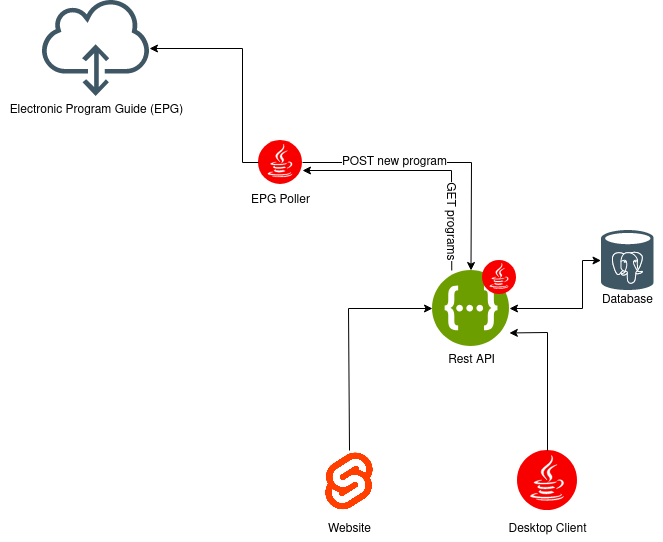
\includegraphics[scale=0.3]{figures/system_logo.png}
\end{figure}

Softwareteknologi\\
\vspace{2mm}
Semesterprojekt 2. semester, ST2-PRO\\
\vspace{2mm}
\textbf{Projektperiode:} 01.01.2020 - 29.05.2020 \\
\vspace{2mm}
\textbf{Afleveringsdata:} 29.05.2020 \\

\vspace{7mm}

\textbf{Projektgruppe 06:} \\
\vspace{2mm}
Jakob Rasmussen, jakra19@student.sdu.dk \\
\vspace{2mm}
Kenneth M. Christiansen kechr19@student.sdu.dk \\
\vspace{2mm}
Kevin K. M. Petersen, kepet19@student.sdu.dk \\
\vspace{2mm}
Kristian N. Jakobsen, kjako19@student.sdu.dk \\
\vspace{2mm}
Mathias N. Rasmussen, mara816@student.sdu.dk \\
\vspace{2mm}
Simon Jørgensen, sijo819@student.sdu.dk \\

\vspace{7mm}

\textbf{Vejleder:} Henrik Lykkegaard Larsen, hlla@mmmi.sdu.dk \\

% Bottom of page
\vfill

Syddansk Universitet\\
Det Tekniske Fakultet\\
Mærks Mc-Kinney Møller Instituttet\\
Campusvej 55, 5230 Odense M

\end{center}
\end{titlepage}
    \newpage
    
    % Titelblad ------------------------------------------------------------------------ Husk at fjerne komment neden under?
    \noindent
\begin{tabular}{@{}l l} 
\textbf{Title:} & Creditoro - Functional \\ 
                & Non-functional Requirements\\
& \\
\textbf{Institution:} & Syddansk Universitet \\
& Det Tekniske Fakultet, Mærsk Mc-Kinney Møller Instituttet \\
& Campusvej 55, 5230 Odense M \\
& \\
\textbf{Uddannelse:} & Softwareteknologi \\
& \\
\textbf{Term:} & 2. term \\
& \\
\textbf{Project group:} & 06\\
& \\
\textbf{Version:} & \texttt{0.0.1-DRAFT}\\
& \\
\end{tabular}

% OwO Jakob Jakob Jakob Jakob Jakob Jakob Jakob Jakob Jakob Jakob Jakob
\vspace{-0.5mm}

\includegraphics[scale=0.07]{figures/signatures/signatureJR.jpg}
\vspace{-9.5mm}
\par\noindent\rule{\textwidth}{0.4pt}
\noindent
Jakob Rasmussen, jakra19@student.sdu.dk\\
% -end- -end- -end -end -end- -end- -end -end -end- -end- -end -end -end-

% Kenneth Kenneth Kenneth Kenneth Kenneth Kenneth Kenneth Kenneth Kenneth
\noindent

\includegraphics[scale=0.3]{figures/signatures/signature_kechr19.PNG}
\vspace{-5mm}
\par\noindent\rule{\textwidth}{0.4pt}
\noindent
Kenneth M. Christiansen, kechr19@student.sdu.dk\\
\vspace{3.5mm}
% -end- -end- -end -end -end- -end- -end -end -end- -end- -end -end -end-

% KEVIN KEVIN KEVIN KEVIN KEVIN KEVIN Kevin Kevin Kevin Kevin Kevin Kevin
\vspace{-6.5mm}
\noindent

\includegraphics[scale=0.3]{figures/signatures/signature_kepet19.png}
\vspace{-8mm}
\par\noindent\rule{\textwidth}{0.4pt}
\noindent
Kevin K. M. Petersen, kepet19@student.sdu.dk
% -end- -end- -end -end -end- -end- -end -end -end- -end- -end -end -end-

% Kristian Kristian Kristian Kristian Kristian Kristian Kristian
\noindent

\includegraphics[scale=0.04]{figures/signatures/signature_kjako19.jpg}
\vspace{-9.5mm}
\par\noindent\rule{\textwidth}{0.4pt}
\noindent
Kristian N. Jakobsen, kjako19@student.sdu.dk\\
% -end- -end- -end -end -end- -end- -end -end -end- -end- -end -end -end-

% Mathias Mathias Mathias Mathias Mathias Mathias Mathias Mathias Mathias
\noindent

\includegraphics[scale=0.120]{figures/signatures/Signatur_mara816.png}
\vspace{-5mm}
\par\noindent\rule{\textwidth}{0.4pt}
\noindent
Mathias N. Rasmussen, mara816@student.sdu.dk\\
% -end- -end- -end -end -end- -end- -end -end -end- -end- -end -end -end-

% Simon Simon Simon Simon Simon Simon Simon Simon Simon Simon Simon Simon
\noindent

\includegraphics[scale=0.042]{figures/signatures/signatureSJ.png}
\vspace{-3.5mm}
\par\noindent\rule{\textwidth}{0.4pt}
\noindent
Simon Jørgensen, sijo819@student.sdu.dk\\
% -end- -end- -end -end -end- -end- -end -end -end- -end- -end -end -end-


%Bottom of page
%\vfill

\noindent
\begin{tabular}{@{}l l}
Number of Pages:    & \pageref{LastPage} pages \\
\end{tabular}

\vspace{3.5mm}

\begin{footnotesize}
\noindent
\textbf{By signing this document every individual group member confirms that they have contributed equally to the project and is thereby liable for the content within this document. }
\end{footnotesize}
    \newpage
 
    % Indholdsfortegnelse
    \tableofcontents
    \newpage
    
    % Start counting from this line
    \pagenumbering{arabic}
    \setcounter{page}{1}

    % Indledning
    \section{Indledning}
Når et program bliver broadcasted på en TV station, skal krediteringer vises. Dette gøres i slutningen af programmet, i maksimalt 30 sekunder. Det betyder, at der ikke altid er tid til at vise alle krediteringer, og derfor prioriteres de før de vises. \\
Hvis de 30 sekunder for hvert program kan frigøres, kan danske TV stationer bruge tiden på at vise noget andet, som f.eks. reklamer. Derved kan TV 2 øge deres årlige indtægter med op til 60 millioner kroner. \\
TV 2 har brug for et system, der kan administrere krediteringer for programmer produceret i Danmark. Hertil skal der kunne tilføjes nye krediteringer i systemet for nye produktioner, samt det skal være muligt at kunne søge efter eksisterende krediteringer. Det skal være muligt at kunne se hvilken rolle en given person har haft i en produktion, da denne person kan have haft flere forskellige roller på flere forskellige produktioner.

\subsection{Projektrammer}
Denne sektion har til formål at opridse rammerne for projektet, samt hvilket område projektgruppen arbejder indenfor.

\subsubsection{Krav til Projektet}
Systemet skal så vidt muligt skrives i programmeringssproget Java. \\
Krediterings-data skal lagres i en database, og i dette projekt skal den brugte database være SQL baseret. Der skal bruges PostgreSQL.\\
Systemet forventes ikke at være et færdigt system, men en række forslag til løsninger der opfylder systembehovet. Forslagene skal inkludere:

\begin{itemize}
    \item Krav
    \item Analyse
    \item Design
    \item Implementering
    \item Test
\end{itemize}

\noindent
Producere der kan tilføje og redigere i krediteringerne, skal kun have mulighed for at redigere i de produktioner, de selv ejer.\\
Det forventes at krediteringssystemet er kompatibelt med andre systemer (f.eks. fra Stofa, YouSee etc.).

\subsubsection{Tidsplan}
Tidsplanen har til formål at skabe overblik og styring over projektet. 
Den giver gruppemedlemmerne et overblik over, hvornår de forskellige dele af projektet skal starte og slutte, og derved bliver det hurtigt klart hvis tidsplanen skrider. \\

\begin{landscape}
    \begin{figure}
        \centering
        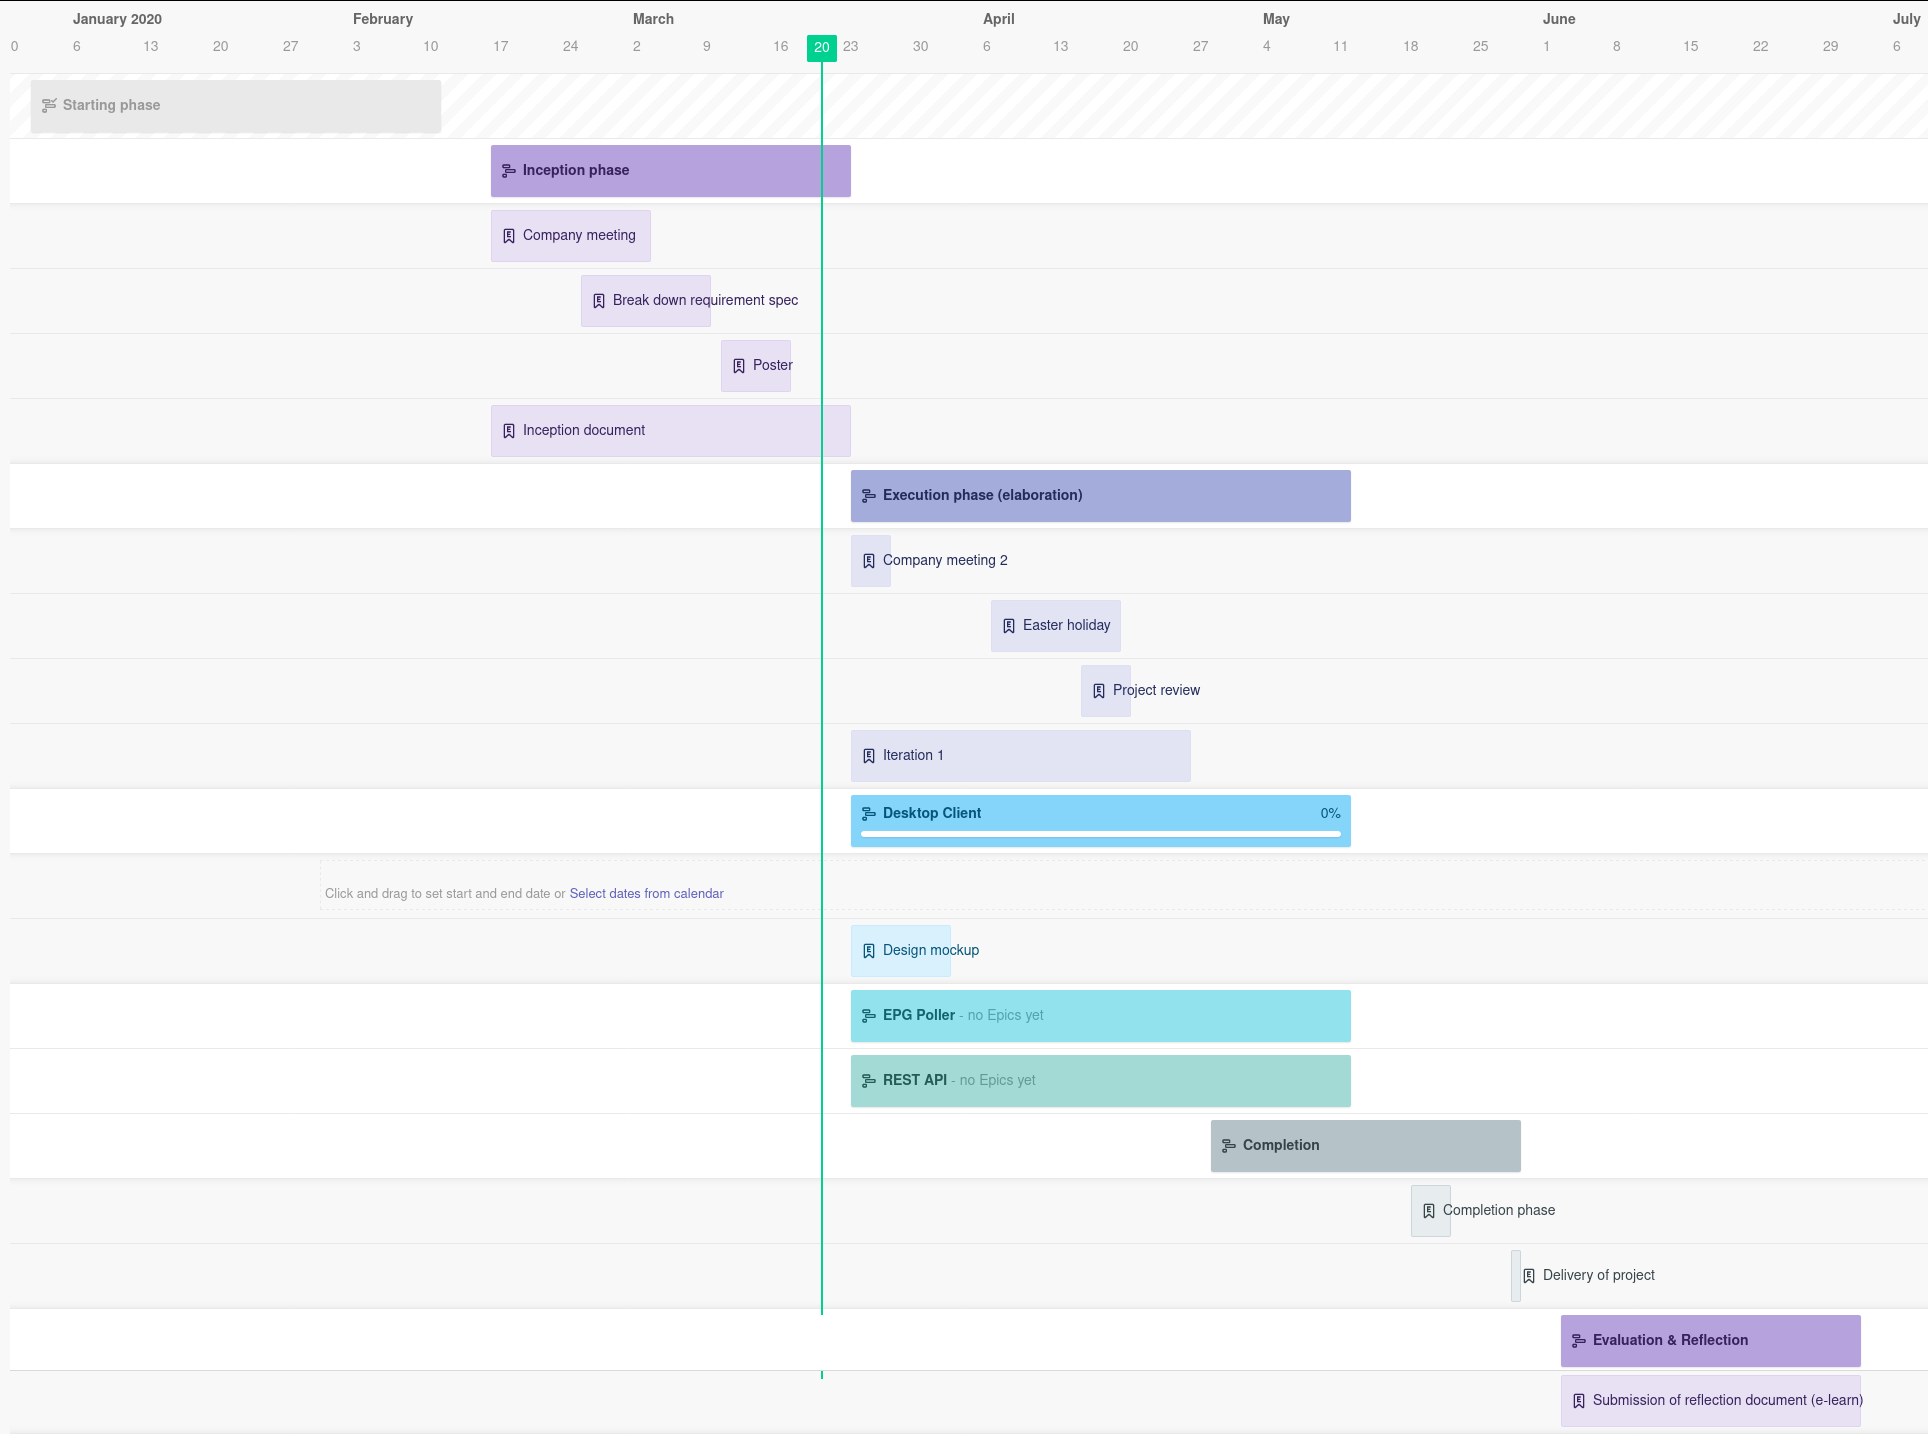
\includegraphics[scale=0.30]{figures/grantt_udvidet.png}
        \caption{Tidsplan for projektet}
        \label{fig:gantt}
    \end{figure}{}
\end{landscape}

% PRE review
% \subsubsection{Hvad ligger uden for projektrammen}
% Der forventes ikke at der laves et produktionsparat system, men et system der kan bruges som et værktøj af TV2. % PRE review: Det er derfor uden for systemets omfang (scope) at lave en REST API.

\subsection{Formål med Inceptionsfasen}
Formålet med inceptionsfasen er at fastlægge systemets omfang, der bliver udformet en overordnet kravspecifikation, kravene prioriteres og metoderne i elaborationsfasen beskrives. Dette sker gennem en nærmere undersøgelse af problemstillingen, indsamling af information og under kundemøder hvor kravene indsamles (eliciteres).\\

\noindent
Målene for inceptionsfasen kan således opstilles i punktform:
\begin{itemize}
    \item At gennemføre kravudvikling
    \item At identificere kritiske risici
    \item At fastlægge projektets metoder i elaborationsfasen
\end{itemize}

\subsection{Problemanalyse}
% PRE review: Hvordan kan vi udvikle et samlet krediteringssystem, der giver mulighed for at erstatte rulletekster efter et endt program?

\subsubsection{Igangsættende Problem}
TV2 ønsker at frigøre 30 sekunders krediterings tekster efter hvert program, så de i stedet kan bruge tiden på at vise reklamer. Problemet består i at disse krediterings tekster, så skal vises på en anden platform.\\

\noindent
I tabel \ref{table:kravFraCase} ses kravene fra TV2's projektcase:

% Oversæt gerne højre kolonne til dansk :-)
\begin{longtable}{|p{12cm}|p{4cm}|}
\hline
\textbf{Beskrivelse} & \textbf{Type} \\
\hline
“Vi har brug for  et krediterings system der kan  håndtere  dansk TV content” 
& En vag opgave \\

\hline
"Dette inkluderer muligheden for at oprette nye krediteringer i systemet, når en ny produktion bliver lavet, samt at have mulighed for at søge efter en given produktion og få en liste af krediteringer, forbundet til denne. Det burde også være muligt at se hvilken rolle en given person har haft i en produktion, eftersom en person kan have flere forskellige roller i forskellige produktioner."
& Ønske om en bestemt løsning \\

\hline 
"Producers/TV-stationer burde være i stand til at redigere krediteringer for programmer/produktioner de ejer. De burde også være i stand til at redigere disse produktioners ID. Systemadministratorer skal kunne vedligeholde (oprette, læse, opdatere og slette) personer, krediteringer og personer."
& Ønske om en bestemt løsning \\

\hline
"Til slut skal systemet kunne offentliggøre en service som andre systemer kan bruge. Disse systemer kan f.eks. være en hjemmeside eller en applikation. Disse andre systemer skal også kunne bruge API'et, så data'et kan blive brugt i allerede eksisterende systemer (såsom TVTID.dk - TV 2's TV-Guide)."
& Ønske om en bestemt løsning \\

\hline
"En form for adgangskontrol skal implementeres, til de beskyttede dele af systemet (oprettelse, opdatering, slettelse, osv. af data)
& Ønske om en bestemt løsning \\

\hline
"Der skal være en offentligt tilgængelig del af systemet, hvor det er muligt at se krediteringer uden at logge ind."
& Ønske om en bestemt løsning \\

\hline
“Nuværende løsning er begrænset til 30 sekunder, og dermed kan alle krediteringerne ikke altid vises i praksis” 
& Et problem \\

\hline
\caption{Krav fra TV2s projektcase}
\label{table:kravFraCase}
\end{longtable}

% -----------------------------------------------------------------------------------------------------
\subsubsection{Identifikation af Problemet}
Som det er nu bliver krediteringer vist i slutningen af et program. Ifølge reglerne for visning af krediteringer, må krediteringer ikke vises mere end 20 sekunder for produktioner under 60 minutter, og 30 sekunder for produktioner over 60 minutter. Dette giver en del problemer. For det første betyder den begrænsede varighed, at ikke alle medarbejdere kan krediteres. Dette ender ud i at der skal prioriteres i krediteringerne, før de bliver vist på TV. Derved får alle medarbejdere ikke den anerkendelse de burde.
Hvis krediteringer flyttes til et eksternt system, og derved ikke bliver vist på TV, kan man undgå at skulle prioritere. Alle kan derved få den fortjente kredit. Derudover vil det også give mulighed for at vise noget andet, som f.eks. reklamer eller promoveringer for andre programmer (red: eget indhold).
\footnote{\href{https://www.dr.dk/NR/rdonlyres/00221a7b/dpikscstjptklixxdnjgywgeuakhwpog/DR_kreditmanual_050810.pdf}{DR’s krediteringsregler for TV}}
% brug bibliography. show me the way

\noindent
Et sådan eksternt system vil også hjælpe med oprettelsen af nye krediteringer, ved at gøre processen hurtigere og nemmere, samt mere overskueligt. Dertil har gruppen valgt at arbejde med samtlige/alle problemstillinger givet af TV2 i tabel \ref{table:kravFraCase}, og lave en prototype til et funktionsdygtigt system. Angående valget med at arbejde med samtlige problemstillinger præsenteret af TV2, har gruppen konkluderet det som værende realistisk jævnfør figur \ref{fig:gantt}. Denne prototype vil kunne bruges som et udkast til et endeligt system.

\subsection{Problemformulering \& Afgrænsning}
\textit{Hvordan kan vi udvikle et samlet krediteringssystem, der giver mulighed for at erstatte rulletekster efter et endt program?}

\begin{enumerate}
    \item Hvem skal kunne håndtere krediteringer?
    \item Hvordan skal krediteringerne gøres tilgængelige, og hvordan skal seerne refereres dertil?
    \item Hvordan kan man oprette et system som kan indeholde krediteringer?
\end{enumerate}

\noindent % afgrænsning
Projektgruppen har valgt at afgrænse dette projekt, ved at konstruere en prototype til et system.
% Indsat post review. 

\noindent % Det vi har med:
Projektgruppen har valgt at lave et system der ligger tæt op ad det oprindelige foreslag fra TV2s projektcase. Dette indebærer alle kravene i tabel \ref{table:kravFraCase}.
\begin{figure}[H]
\centering
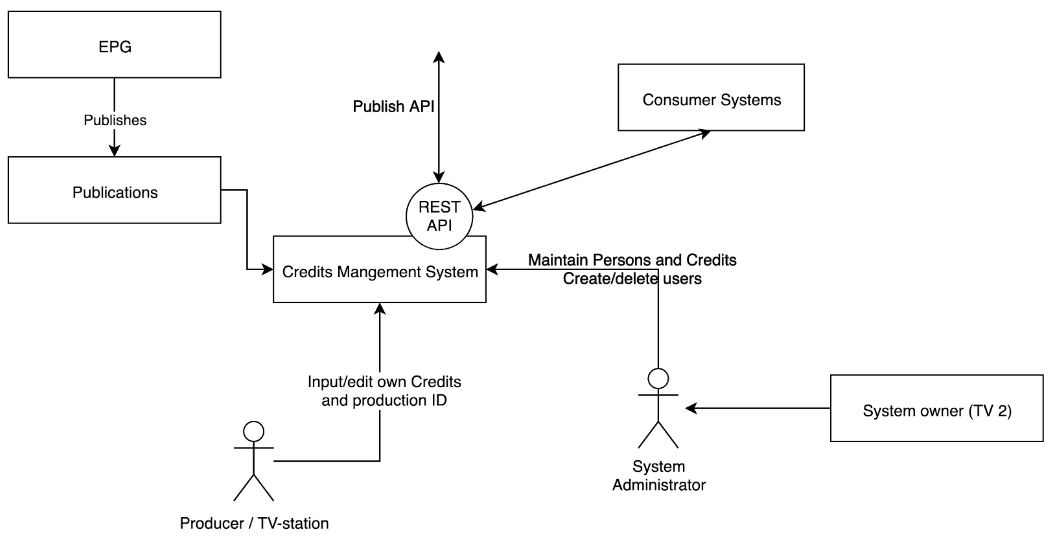
\includegraphics[scale=0.3]{figures/tv2_system.png}
\label{fig:tv2_system}
\caption{Foreslag til systemtegning - © TV2}
\end{figure}
% Indsæt figur af deres oprindelige systemtegning?

\noindent % Det vi vælger fra:
I et produktionsklart system vil det være ideelt at have en webside, men dette har vi konkluderet som værende uden for projektet.
    \newpage
    
    % Faglig vidensgrundlag
    \section{Faglig Vidensgrundlag}

\subsection{Begrebsdefinitioner} 
De begreber der findes i denne rapport er defineret i tabel \ref{tab:Begrebsdefinitioner}:

% Begrebsdifinitioner
\begin{table}[h]
    \centering
\begin{tabular}{|p{4cm}|p{12cm}|}
\hline
\textbf{Begreb} \& \textbf{Definition} \\
\hline
REST API    & REST: \\
            & Repræsentativ tilstandsoverførsel (dansk oversættelse af REST) er en software-arkitektonisk stil, der definerer et sæt begrænsnigner, der skal bruges til at oprettelse af webtjenester\\
            & API: \\
            & API står for Application Programming Interface, og er en softwaregrænseflade, der tillader et stykke software at interagere med andet software \\
\hline
EPG         & EPG er en forkortelse for Electronic Programme Guide. Det er en generelt betegnelse for elektronisk programoversigt over TV-programmer         \\
\hline
GDPR        & Databeskyttelsesforordning, der har til formål at styrke og harmonisere beskyttelsen af personoplysninger i EU \\
\hline
SQL         & Structured Query Language er et programmeringssprog til relationelle databaser\\
\hline
Person & Person er de medarbejdere der skal krediteres. Det kunne f.eks. være en skuespiller eller en lydmand. \\
\hline
Personinformation & Personlig information som fx e-mail, tlf. nr. osv. \\
\hline
Swagger UI  & Brugergrænseflade til vores REST Api. (\url{https://swagger.io/}) \\
\hline
Docker      & Bruges til containeriseringen, så host styresystemet bliver agnostisk, og softwaren bliver indkapslet. Det forhindrer også "it works on my machine" problemer.  \\
\hline
 \end{tabular}
    \caption{Begrebsdefinitioner}
    \label{tab:Begrebsdefinitioner}
\end{table}

% Fagligt Videngrundlag ----------------------------------------------------------------------------
\subsection{Fagligt Vidensgrundlag}
Dette afsnit har til formål at dækker over den faglige viden gruppen skal have, for at kunne udføre projektet.

\subsubsection{JAVA}
At have kendskab til Java er en vigtig forudsætning for udarbejdelsen af projektet. Systemet vil hovedsageligt blive programmeret i sproget Java. Det faglige niveau svarer til 2. semesterstuderende på Softwareteknologi. Dette indebærer blandt andet forståelse af JavaFX og Scenebuilder.
Arbejdet med Java i projektet forudsætter derudover forståelse for basale programmeringsprincipper og forståelse for det objektorienterede programmeringsparadigme. 

\subsubsection{Python}
Et grundlæggende kendskab til Python kræves for at kunne forstå - samt implementere REST Api'et.

\subsubsection{Database}
Systemet vil indeholde en lang række data, som skal lagres i en database. Det er derfor nødvendigt at have forståelse for databaser, databasestrukturer, relationelle SQL-databaser og SQL-queries. Databasen der vil blive benyttet i projektet er PostgreSQL, en basal viden om databasesproget/programmeringssproget SQL er derfor nødvendig. 
Al nødvendig viden er givet i SDU's 'Data Management' kursets pensum.

\subsubsection{Ubuntu \& Docker}
En basal forståelse for Ubuntu (eller andet Linux baseret distro) og Docker kræves for opsætning af REST Api'et og databasen.

\subsection{Relevante Eksisterende Løsninger}
\textbf{IMDb} \\
IMDb (Internet Movie Database) er en online database bestående af film, serier, medvirkende m.m. Man har mulighed for at søge efter informationer ved at referere til blandt andet førnævnte titler. IMDb har også et ratingsystem, der gør det muligt at bedømme film, serier etc.
\textbf{Rotten Tomatoes} \\
Rotten Tomatoes er på lige fod med IMDb, en database for film, serier, medvirkende m.m. Man kan på Rotten Tomatoes også søge information. Rotten Tomatoes distancerer sig fra IMDb, ved både at tage ratings fra sine brugere og et panel af anmeldere. 


    \newpage
    
    % Overordnet kravspecifikation
    \section{Overordnet Kravspecifikation}

\noindent
Systemet afspejler det system TV2 har lagt op til i projektcasen. Der er tale om et system, hvor alle kan se - og nogle kan redigere krediteringer for programmer. Systemet skal kunne tilgås via en dansk brugergrænseflade. Det skal indeholde forskellige brugerroller; systemadministrator, kanaladministrator, producer, royalty bruger og gæst.\\

\noindent
Systemadministratoren skal have rettigheder til at gøre alt. Dette gælder f.eks. at oprette krediteringer, kanaladministratorer og producerer. Kanaladministratoren skal kunne redigere, oprette og slette krediteringer for egen kanal. En producer skal kunne tilføje og redigere i krediteringerne for egne produktioner, og en gæst skal kunne se krediteringer for alle programmer. 
Det skal være muligt at kombinere personer som refererer til den samme person i den virkelige verden. Når to forskellige producere vil oprette en kreditering for et program, skal krediteringen være associeret med en person og vedkommendes rolle. Det betyder altså, at det skal være muligt at oprette personer der kan sammenflettes (f.eks. med UUID).\\

\noindent
TV2 har ikke lov til at lagre persondata, såsom et CPR-nummer eller et telefonnummer, så det skal være muligt at identificere personer i systemet og sikre at krediteringerne er korrekt forbundet til de rigtige personer.
Det skal være muligt at eksportere en specifik mængde data i forskellige formater såsom XML og CSV. Derudover skal databasen være søgbar, så det er nemt at finde personer, programmer og lignende. Det er vigtigt at systemet er nemt at bruge, så seerne nemt kan se krediteringerne for det program de lige har set.\\

\noindent
TV 2 kunne være interesseret i at integrere systemet med andre systemer (YouSee Tv, Boxer Play osv.), og det er derfor vigtigt at systemet er kompatibelt med krediteringer i andre systemer. Det kunne også være interessant at have muligheden for at få notifikationer når noget nyt sker i systemet. Samrådet for Ophavsret og Producentforeningen kunne også være interesseret i at modtage en form for meddelelse hver gang der er blevet tilføjet noget nyt til systemet, hvor de kan godkende krediteringerne og ud fra disse udbetale royalties. Derudover kunne det også være interessant at brugergrænsefladen kunne undestøtte flere sprog.\\

\noindent
For at beskytte dele af systemet (tilføjelse/redigering/sletning af data osv.), skal der indføres en form for adgangskontrol. Der skal være en offentligt tilgængelig del af systemet, hvor det er muligt at se krediteringerne for et et program uden at skulle logge ind.\\

\noindent
I tabel \ref{table:kravliste} ses kravene opsummeret i en tabel for bedre overblik.

\begin{longtable}[h]{ |p{1cm}|p{4cm}|p{11cm}| }

\hline
\textbf{ID} & \textbf{Navn} & \textbf{Beskrivelse} \\
\hline
K01 & Brugergrænseflade & Systemet skal tilgås via en dansk brugergrænseflade \\
\hline
K02 & Brugerroller & Systemet skal indeholde brugerroller \\
\hline
\label{K03}K03 & Tildel roller & Kanaladministrator skal kunne tildele producer- og kanaladministrator roller \\
\hline
K04 & Slet bruger & Systemadministratoren skal kunne slette brugere \\
\hline
K05 & Se krediteringer & Alle skal kunne se krediteringer \\
\hline
K06 & Søg efter krediteringer & Alle skal kunne søge efter og se krediteringer for alle programmer \\
\hline
K07 & Opret krediteringer & Specielle brugere, kanaladministratore og systemadmin skal kunne oprette
krediteringer for et givent program \\
\hline
K08 & Rediger krediteringer & Specielle brugere, kanaladmin og systemadmin skal kunne redigere krediteringer for egne programmer \\
\hline
K09 & Slet kreditering & Kanaladmin og systemadmin skal kunne oprette/redigere/slette krediteringer under egen kanal \\
\hline
K10 & Søg efter personer & Alle skal kunne søge efter personer \\
\hline
K11 & Knyt personer til krediteringer & Personer skal kunne knyttes til krediteringer så man kan se hvilke programmer en person har deltaget i Systemadmin, kanaladmin og producer skal kunne se persondata som email og tlf. nr. \\
\hline
K12 & Link personer i den virkelige verden & Det skal være muligt at linke personer i krediteringer til personer i den virkelige verden, så der krediteres korrekt \\
\hline
K13 & Eksporter data & Brugere skal kunne eksportere data til forskellige formater såsom XML og CSV \\
\hline
K14 & Importering af data & Systemet skal kunne importere EPG data via TVTid.dk \\
\hline
K15 & Integration & Systemet skal kunne integreres med andre systemer (Yoursee Play, Boxer Play, osv.) \\
\hline
K16 & Notifikationer & Systemet skal sende notifikationer til relevante brugere \\
\hline
K17 & Sprogvalg & Systemet skal kunne understøtte flere sprog \\
\hline
\caption{Liste af krav fra overordnet kravspecifikation} 
\label{table:kravliste}
\end{longtable} 

\subsection{Aktørliste}
Aktørlisten er sat op sådan, at overaktøren har samme rettigheder som underaktøren, samt ekstra rettigheder. F.eks. har systemadministratoren samme rettigheder som kanaladministratoren, plus rettigheder til at oprette kanaler, slette personer osv.\\


\begin{longtable}{|p{3.7cm}|p{6.15cm}|p{6.15cm}|}
\hline
\textbf{Aktør} & \textbf{Beskrivelse} & \textbf{Mål \& tjenester} \\
\hline
Systemadministrator (p) 
& Systemadministratoren har samme rettigheder som alle andre aktører. Denne aktør står primært for at slette personer, samt at oprette og slette kanaler. Til disse kanaler skal systemadministratoren tildele kanaladministratorroller.
& - Slette personer \newline - Oprette og slette kanaler \newline - Tildele og fjerne kanaladministratorroller\\

\hline
Kanaladministrator (p) 
& Kanaladministratoren skal godkende nyoprettede krediteringer, og har rettigheder til at slette krediteringer under egen kanal. Kanaladministratoren står får at tildele producer- og andre kanaladministratorroller for egen kanal.
& - Godkende nyoprettede krediteringer \newline - Slette krediteringer under egen kanal \newline - Tildele producer- og kanaladministratorroller for egen kanal\\

\hline
Royalty bruger (p) 
& Royalty bruger repræsenterer firmaer, som Registrering Danmark, der sørger for at betale royalties til medarbejdere på produktioner.
& - Kan eksportere data \\

\hline
Producer (p) 
& Produceren for et program står for at oprette nye krediteringer, samt rette krediteringer for egne produktioner.
& - Kan oprette krediteringer \newline - Kan redigere i eksisterende krediteringer for egne produktioner \newline - Kan logge ind og af \newline - Kan se personinformation \\

\hline
Gæst (p) 
& Gæsten repræsenterer offentligheden, som skal kunne søge efter informationer og krediteringer om forskellige programmer samt personer. Gæsten kan se alle produktioner en person har været med i. Gæsten kan også ændre sproget for brugergrænsefladen.
& - Kan søge efter og se krediteringer og personer for forskellige programmer \newline - Se alt hvad en person har været med i \newline - Ændre sproget\\

\hline
\caption{Aktørlisten}
\label{table:aktørlist}
\end{longtable}

\subsection{Overordnet Brugsmønstermodel}

\begin{figure}[H]
    \centering
    \captionsetup{justification=centering}
    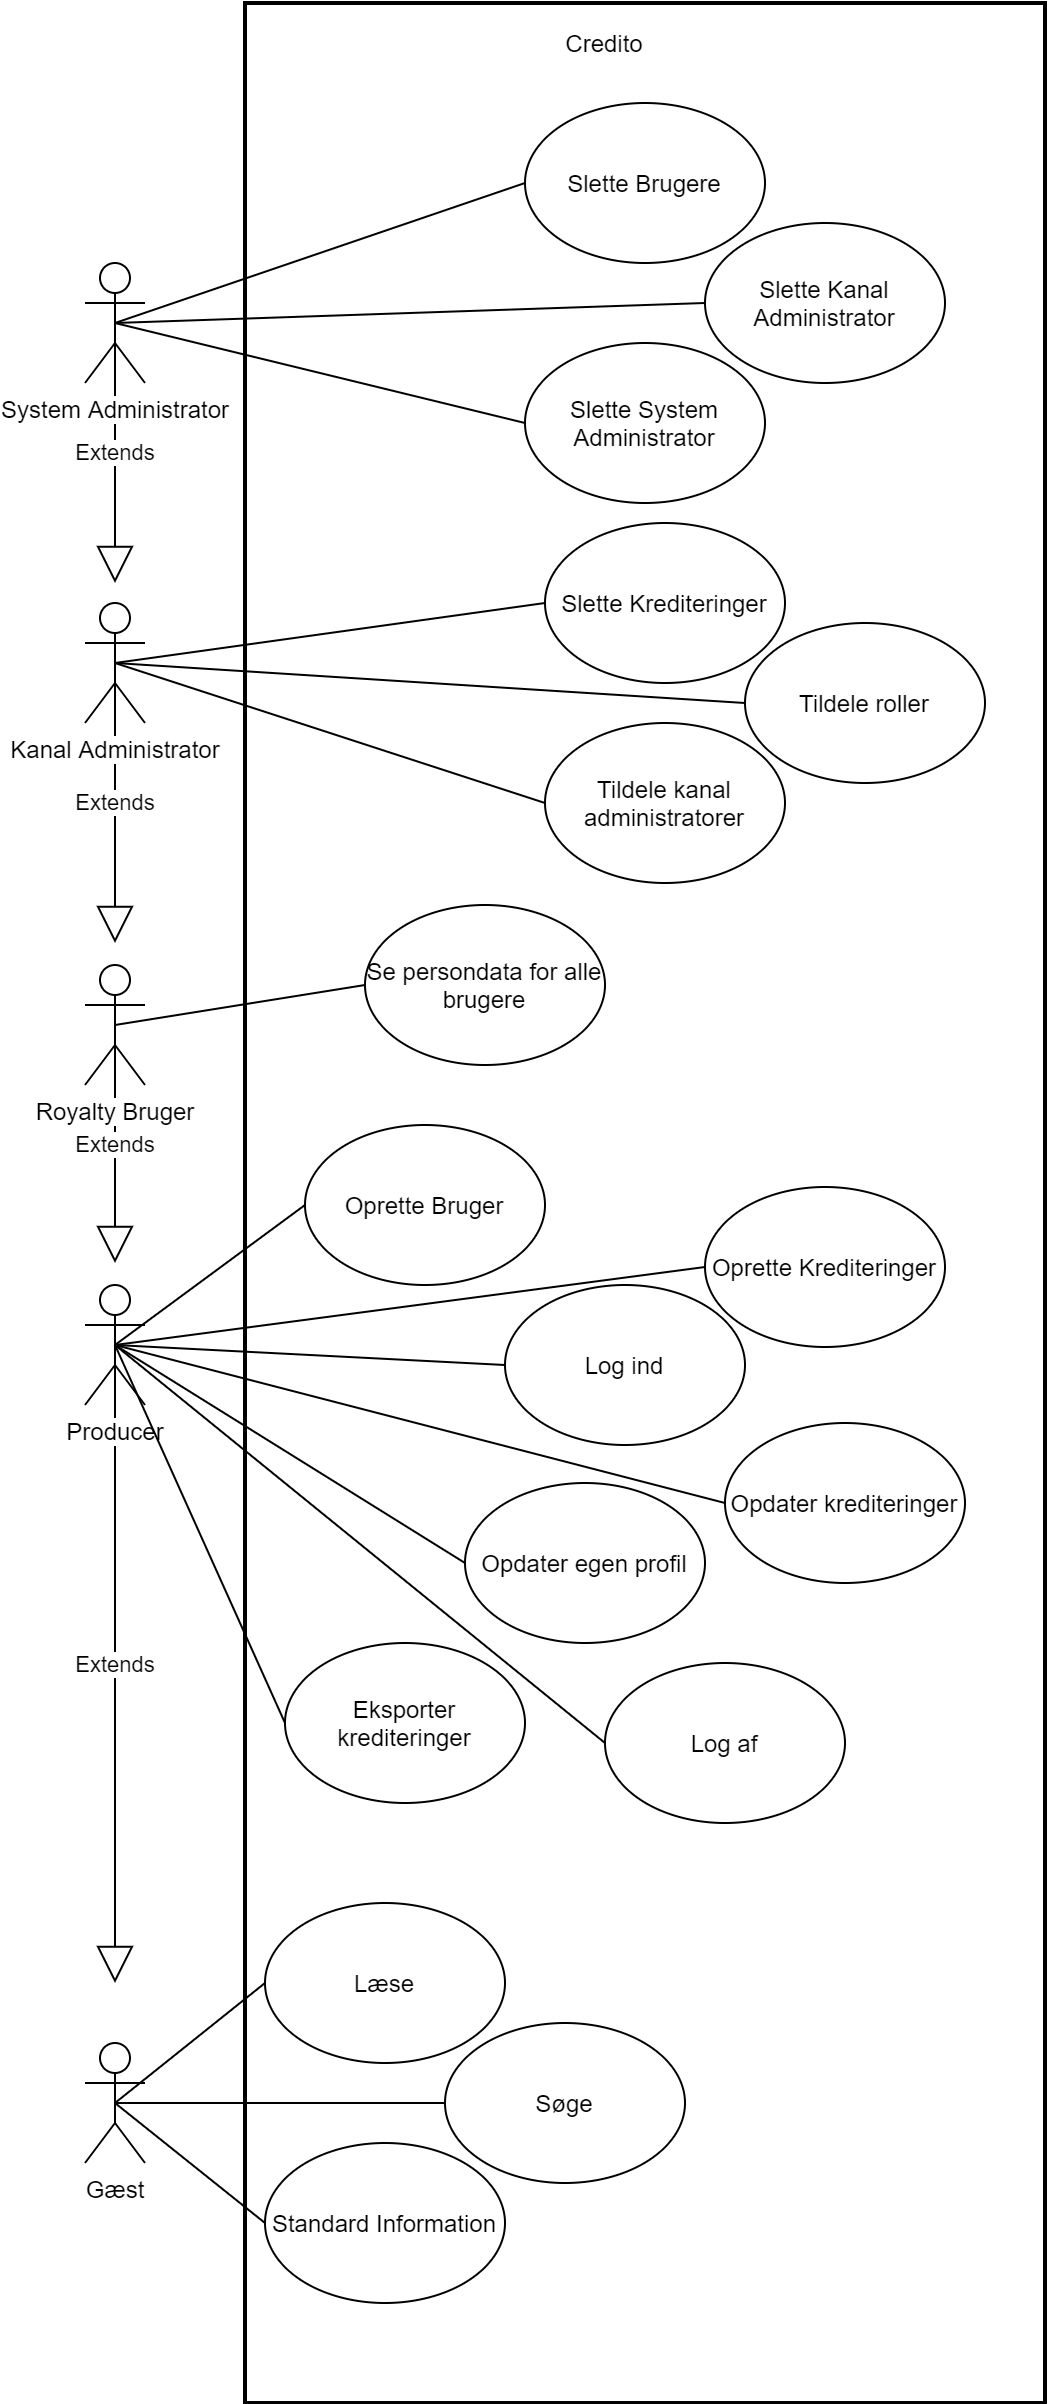
\includegraphics[scale=0.22]{figures/use-case.png}
    \caption[Overordnet brugsmønster over Creditoro systemet]%
    {Overordnet brugsmønster over Creditoro systemet 
    \par \small Menneskene er aktører. \\
    \small Cirklerne beskriver handlinger aktørne kan lave. \\
    \small Pilende betyder Extends, hvilket vil sige aktørerne arver funktionalitet}
    \label{fig:usecasemodel}
\end{figure}

\newpage
\subsection{Liste over Brugsmønstre}

\begin{longtable}[h]{|p{0.6cm}|p{6.4cm}|p{9cm}| }
\hline
\textbf{ID} & \textbf{Navn} & \textbf{Aktør} \\
\hline
B01 & Opdater egen royalty bruger & Systemadministrator (p), Royalty Bruger (p) \\
\hline
B02 & Opdater person & Systemadministrator (p), kanaladministrator (p), producer (p) \\
\hline
B03 & Opret Producer & Systemadministrator (p), kanaladministrator (p) \\
\hline
B04 & Opret person & Systemadministrator (p), kanaladministrator (p), Producer (p) \\
\hline
B05 & Fjern producer & Systemadministrator (p) \\
\hline
B06 & Fjern person & Systemadministrator (p) \\
\hline
B07 & Opret kreditering & Systemadministrator (p), Kanaladministrator (p), producer (p) \\
\hline
B08 & Fjern kreditering til program & Systemadministrator (p), kanaladministrator (p) \\
\hline
B09 & Opdater egne kreditering & Systemadministrator (p), kanaladministrator (p), Producer (p) \\
\hline
B10 & Læse krediteringer & Systemadministrator (p), kanaladministrator (p), Royalty Bruger (p), Producer (p), Gæst (p) \\
\hline
B11 & Se person profil & Systemadministrator (p), kanaladministrator (p), Royalty bruger (p), Producer (p), Gæst (p) \\
\hline
B12 & Søge efter personer og programmer & Systemadministrator (p), kanaladministrator (p), Royalty Bruger (p), Producer (p), Gæst (p) \\
\hline
B13 & Log ind & Systemadministrator (p), kanaladministrator (p), Royalty Bruger (p), Producer (p) \\
\hline
B14 & Log af & Systemadministrator (p), kanaladministrator (p), Royalty Bruger(p), Producer (p) \\
\hline
B15 & Kan se personinformation & Systemadministrator (p), kanaladministrator (p), Royalty Bruger (p), Producer (p) \\
\hline
B16 & Godkende nye krediteringer & Systemadministrator (p), Kanaladministrator (p) \\
\hline
B17 & Afvise nye krediteringer & Systemadministrator (p), Kanaladministrator (p) \\
\hline
B18 & Opret kanaladministrator & Systemadministrator (p), kanaladministrator (p) \\
\hline
B19 & Opret systemadministrator & Systemadministrator (p) \\
\hline
B20 & Ændre sprog & Systemadministrator (p), kanaladministrator (p), Royalty Bruger (p), Producer (p), Gæst (p) \\
\hline
\caption{Brugsmønstre}
\label{tab:brugsmønstre}
\end{longtable}

\newpage
\subsection{Overordnet Supplerende Krav}

Her bruges FURPS for supplerende krav.
\begin{table}[H]
    \centering
    \begin{tabular}{|p{3cm}|p{13cm}|}
    \hline
    \textbf{FURPS}           &    \textbf{Krav} \\
    \hline
    %What the customer wants! Note that this includes security-related needs.
    Functionality           & Skal kunne kreditere produktionsroller som er angivet af DRs Krediteringsregler \\
                            & Skal overholde GDPR \\
    \hline
    % How effective is the product from the standpoint of the person who must use it? Is it aesthetically acceptable? Is the documentation accurate and complete?
    Usability       & Systemet skal kunne understøtte flere sprog \\
    \hline
    % What is the maximum acceptable system downtime? Are failures predictable? Can we demonstrate the accuracy of results? How is the system recovered?
    Reliability     &  Hvis serveren til systemet genstarter, startes del-systemerne igen automatisk. Der vil ikke være behov for at ligge systemet ned regelmæssigt for at kunne foretage backup. \\
    \hline
    % How fast must it be? What's the maximum response time? What's the throughput? What's the memory consumption?
    Performance     &  Databasen skal kunne håndtere 10000 nye brugere - samt 15000 krediteringerer årligt i 25 år, uden at ofte brugte kald til REST Api'et bliver sløvt (reponsetid på mere end 300 ms) \\
    \hline
    % Is it testable, extensible, serviceable, installable, and configurable? Can it be monitored?
    Supportability  &  Systemet vil indeholde unit tests, og komme med en rapport over hvor stor en procendel der er dækket af dette. % Hvis der er mere tid kan vi indrage integrations tests?
    %Centraliseret logning (Elastic search, eller blot centraliseret system log?)
    Systemet vil blive forbundet til det centraliserede fejllognings system \texttt{Sentry}.
    Systemet er installerbart vha. Docker via Docker-compose. % (så vi blot kan sige docker-compose up -d for at få systemet op).
    Det vil være muligt at konfigurere system indstillinger via en \texttt{.env} (miljø) fil.
    En opsætningsguide vil være at finde sammen med kildekoden. 
    \\ \hline
    % The + reminds us of a few additional needs that a customer could have:
    % fx. Design constraints, Implementation requirements, interface requirements or physical requirements.
    \end{tabular}
    \caption{FURPS}
    \label{tab:furps}
\end{table} 


\subsection{Detaljerede Beskrivelse af Udvalgte Essentielle Brugsmønstre}
Ud fra MoSCoW har vi valgt 2 brugsmønstre vi mener er essentielle for systemet. De to brugsmønstre er 'Læs kreditering' og 'Opret kreditering'. Til disse to brugsmønstre har vi lavet detaljerede brugsmønstre som kan ses i tabel \ref{table:read_credits} og tabel \ref{tab:create_credits}.

\begin{longtable}[h]{|p{16cm}|}
    \hline
    \textbf{Brugsmønster:}  Læs kreditering \\ 
    \hline
	\textbf{ID:} UC10 \\ 
	\hline
	\textbf{Primære aktører:} Systemadministrator, kanaladministrator, producer, royalty bruger, gæst \\ \hline
	\textbf{Sekundære aktører:} \\ \hline
	\textbf{Kort beskrivelse:} Alle skal kunne se krediteringen for programmerne. \\ \hline
	\textbf{Prækonditioner (Pre conditions):} \\ \hline
\textbf{Hovedhændelsesforløb (main flow):} \\
1. Brugsmønstret starter når en aktør vil se kredit for et program \\
2. Aktøren søger efter programmet \\
3. Aktøren trykker på det ønskede program \\
4. Systemet checker hvilken rolle aktøren har \\
5. Aktøren bliver omdirigeret til den passende visning af krediteringen \\ \hline
    \textbf{	Postkonditioner (post conditions):} \\
    En kreditering bliver vist \\ \hline

	\textbf{Alternative hændelsesforløb (alternative flow):} \\
Step 2: Hvis programmet ikke findes, får vedkommende besked om at programmet ikke findes \\ 
\hline
\caption{Brugsmønster: Læs kreditering}
\label{table:read_credits}
\end{longtable}

% Kevin something fishy here
% Skal det ikke være tabular?
\begin{longtable}[h] {|p{16cm}|}
\hline
    \textbf{Brugsmønster:} Opret kreditering \\
    \hline
	\textbf{ID:} UC07 \\ \hline
	\textbf{Primære aktører:} Systemadministrator, kanaladministrator, Producer \\ \hline
	\textbf{Sekundære aktører:} \\ \hline
	\textbf{Kort beskrivelse:} Produceren opretter en kreditering. Heri angives alle der har bidraget til produceringen af TV-programmet, filmen el. lign. \\ \hline
	\textbf{Prækonditioner (Pre conditions):} \\
Aktøren skal være logget på systemet \\ \hline
\textbf{Hovedhændelsesforløb (main flow):} \\
	1. Brugsmønstret starter når en administrator eller producer vil oprette en kreditering \\
	2. Aktøren trykker på knappen ‘Opret Kreditering’ \\
	3. Systemet checker aktørens rolle \\
	4. Aktøren er forbundet til en kanal, og angiver programmets titel \\
	5. Systemet checker om der allerede findes et program med den angivne \\ titel
	6. Aktøren krediterer alle der har medvirket i produktionen af \\ programmet
	7. Aktøren sender den færdige kreditering videre til godkendelse \\
	8. Postkonditioner (post conditions): \\
	9. En kreditering er blevet oprettet \\ \hline
	\textbf{Alternative hændelsesforløb (alternative flow):} \\
Step *: Aktøren kan til enhver tid afbryde oprettelsen af krediteringen \\
Step 4: Hvis aktøren er systemadministrator, er vedkommende ikke forbundet til en kanal, og kan skifte hvilken kanal krediteringen skal oprettes ved. \\

Step 5: Hvis programmets titel allerede eksistere, gøres aktøren opmærksom på dette. \\

Step 8: Hvis krediteringen afvises, laves de fornødne ændringer, og den nye kreditering sendes videre til godkendelse. \\
\hline
\caption{Brugsmønster: Opret kreditering}
\label{tab:create_credits}
\end{longtable}
    \newpage

    % Kritiske risici
    \section{Kritiske Risici}

\noindent
Nedenfor ses en tabel med de fem identificerede risici. 'Risikovurdering' vurderer hvor høj sandsynligheden er for at de identifererede risici indtræffer. 'Indvirkning' vurderer hvor meget det vil påvirke projektet, hvis risikoen bliver en realitet. 'Håndtering' sætter en mulig handlingsplan, såfremt risikoen bliver aktuel. 'Kritisk?' vurderer om risikoens indtræf er kritisk for projektet.



\begin{longtable}[h]{|p{2cm}|p{2.2cm}|p{1.6cm}|p{7cm}|p{1.5cm}|}
    \hline
    \textbf{Risiko}                 &  \textbf{Risikovurd.}     &   \textbf{Indvirk.}    &   \textbf{Håndtering}         &   \textbf{Kritisk?}\\
    \hline
    COVID-19                    &   Høj                         &   Høj                     &   I tiden under hjemmekarantænen, vil al skolerelateret arbejde, inkl. undervisning, foregå online. For at undgå komplikationer, stilles der højere forventninger til at udleveret læsning fra undervisningen vil blive nærstuderet, samt at al undervisning følges så godt som muligt. Vejleder står til rådighed på mail såfremt presserende spørgsmål skulle opstå            &   Ja \\
    \hline
        REST API                    &   Middel-høj                  &   Høj                     &   Der vil fra starten af projektets construction fase af være ekstra fokus på, om det er realistisk at nå at lave REST-API'et. Øjeblikket gruppen vurderer det ikke er muligt, vil REST-API'et blive droppet, og gruppens SCRUM board vil i fællesskab blive opdateret.            &   Ja \\
    \hline
        Tidsplan overholdes ikke    &   Middel-høj                  &   Høj                     &   Overholdes tidsplanen ikke, vil der blive kigget på de aktuelle arbejdsopgaver, og alt efter om arbejdsbyrden er for stor eller lille, vil der blive tilpasset derefter.            &   Ja \\
    \hline 
        Systemet møder ikke kravene &   Lav                         &   Høj                     &   Hvad kunne gøres anderledes? Hvad kan der gøres fremadrettet for at opnå et mere tilfredsstillende resultat. Gruppen perspektiverer samlet             &   Ja \\
    \hline
        Mistet medlem               &   Lav                         &   Middel-høj              &   Et mistet medlem vil lede til manglende arbejdskraft. Arbejdsbyrden/arbejdsopgaverne vil derfor blive opdateret, til de nye gruppeforhold.            &   Ja \\
    \hline
    \caption{Kritiske risici}
    \label{tab:risks}
\end{longtable}
    \newpage
    
    % Prioritering
    \section{Prioritering}
\subsection{Forretningsmæssige Betydning}
% MoSCW: I hvor høj grad er kravet forretningsmæssigt kritisk?
Til prioriteringen af brugsmønstrene er MoSCoW metoden benyttet. Resultatet kan ses nedenfor på figur \ref{fig:moscow}.\\

\begin{figure}[h]
\centering
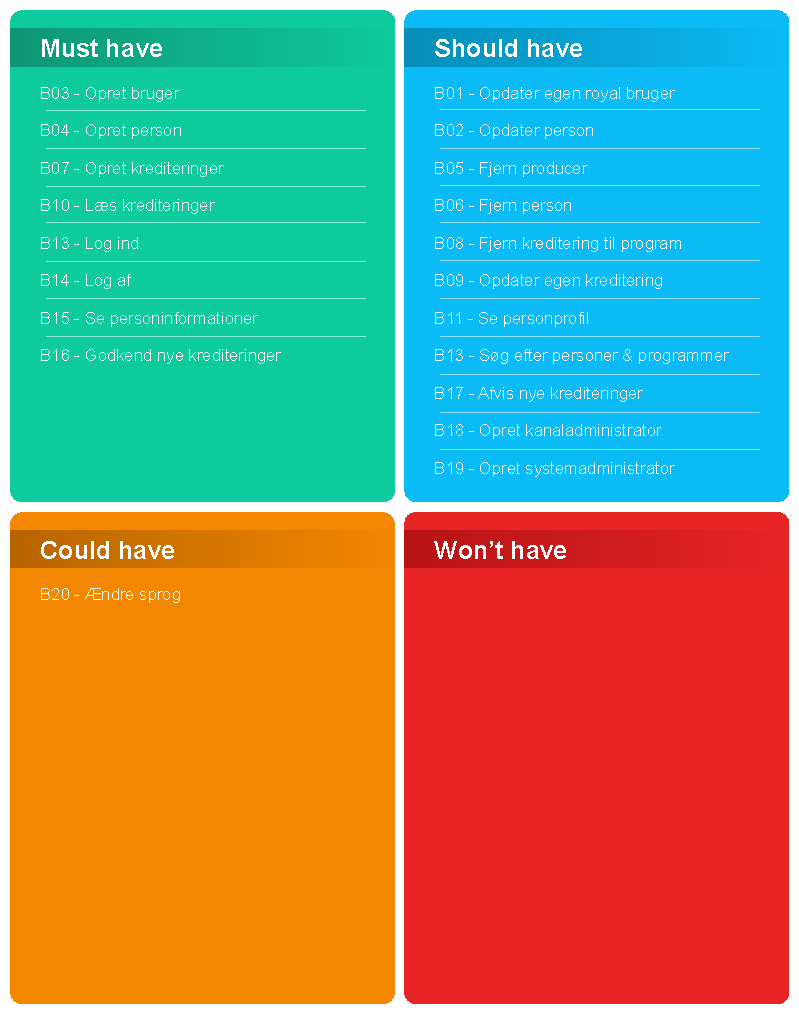
\includegraphics[scale=1]{figures/MoSCoW.pdf}
\caption{MoSCoW}
\label{fig:moscow}
\end{figure}

\noindent
Her ses de forskellige brugsmønstre I en MoSCoW. MoSCoW bruges til at finde ud af hvad der skal udvikles først. 
Da der ikke blev fundet ting i Inceptionsfasen, som der ikke skulle med dennegang, kom der ikke noget i "Won't have" sektionen.

\subsection{Arkitektonisk Betydning}

\noindent
De arkitektoniske krav der har en arketeknoisk betydning for systemet er:
\begin{itemize}
    \item Brugergrænsefladen til klienterne vil være på Dansk.
    \item Brugergrænsefladen(Swagger UI) til REST Api'et vil være på Engelsk.
    \item Persistens vil blive håndteret af en database
    \item Databasen vil være PostgreSQL
    \item Systemet vil automatisk starte efter evt. server genstart.
\end{itemize}
% Hvis vi arbejder med dette krav, vil det så i særlig grad hjælpe os til at få udviklet en passende løsningsstruktur?
% Som jeg forstår dette, bør vi se på alle vores funktionelle/ikke funktionelle krav, hvis kravet bidrager til en bedre løsningsstruktur, angiv kravet og fortæl hvordan.


%\subsection{Risiko} UNDLADET
% Hvis vi arbejder med dette krav, vil det så i særlig grad hjælpe os med at få håndteret risici?
% Som jeg forstår dette, bør vi se på alle vores funktionelle/ikke funktionelle krav, hvis kravet mindsker risici, nævn det.

\subsection{Læringsmæssige Udbytte}
% Hvis vi arbejder med dette krav, vil vi så i særlig grad opnå et læringsmæssigt udbytte?
% Som jeg forstår dette, bør vi se på alle vores funktionelle/ikke funktionelle krav, hvis kravet giver os en særlig grad af læringsmæssigt udbytte.
\begin{itemize}
    \item Supplerende krav - REST Api
    \begin{itemize}
        \item Vi har lagt op til et system der vil afspejle den løsning som TV2 oprindeligt lagde op til. Den løsning indeholder et REST Api, som er vurderet som værende udenfor det der forventes at kunne som studerende på nuværende tispunkt. Ved at vælge sådan en løsning, vil det give os et rigtigt godt redskab i vores programmerings-værktøjskasse i fremtidige projekter.
    \end{itemize}{}
\end{itemize}


\subsection{X-faktor}
% Handler dette krav om noget som vi vil finde særligt motiverende, spændende, sjovt ... at arbejde med?
\begin{itemize}
    \item \myworries{Der mangler reference til funktionkrav 14 - doobelt klip på mig og kig ned}
    \item \hyperref[table:funktionskrav]{K14 - Importering af data} 
    \begin{itemize}
        \item Integrationen mellem andre systemer, og gå de forskellige systemer til at spille sammen er spændende. Det er her med til at give systemet et løft, da det automatiserer oprettelsen af nye programmer i systemet.
    \end{itemize}{}
\end{itemize}


    \newpage
    
    % Metode i elaborationsfasen
    \section{Metoder \& Værktøjer}
\subsection{Metoder i Inceptionsfacen}
\subsubsection{Brugsmønsterdiagram}
Det første skridt i udviklingen af et brugsmønster er at finde og definere de forskellige aktører der vil interagere med systemet. En aktør kan defineres som alt der kommunikerer med systemet og ikke selv er en del af systemet. Et eksempel på dette kunne være en kunde på en webshop. Disse aktører opstilles i en tabel sammen med de brugsmønstre hver aktør kan tilgå. \\

\noindent
Da kravindsamling er en evolutionær aktivitet, bliver alle aktører ikke nødvendigvis identificeret i første iteration. Det er muligt at identificere primærer aktører i løbet af første iteration, og først senere i forløbet blive i stand til at identificere sekundære aktører, når man får mere viden om systemet. \textit{Primære} aktører interagerer med systemet for at opnå påkrævede systemfunktioner, og ud fra det, få noget ud af at bruge systemet. \textit{Sekundære} aktører støtter systemet så de primærer aktører kan gøre deres arbejde. Når aktørerne er fundet kan brugsmønstrene findes. Et brugsmønster angiver et scenarie en aktør kan interagere med. \\

\noindent
Når både aktører og brugsmønstre er fundet, kan man opstille et brugsmønster-diagram for at give en visuel forståelse for hvilke aktører der kan tilgå hvilke brugsmønstre. Et eksempel på et brugsmønsterdiagram kan ses på figur \ref{fig:usecasemodel} \\

\noindent
Brugsmønstermodellen hjælper udvikleren med at forstå brugeren, så systemet kan konstrueres. Idet der er et samlet billede af hvordan systemet skal se ud, vil udviklingen være mere målfast da kravene og deres forhold til brugeren er klare.

\subsubsection{FURPS}
FURPS er en model til klassificering af ikke-funktionelle krav, og er med til at give en detaljeret beskrivelse af kravene. Akronymet står for:

\noindent
\begin{description}
    \item [Functionality:] Hvad kunden vil have. Dette inkluderer også sikkerhedsforanstaltninger.
    \item [Usability:] Hvor effektivt er produktet fra brugerens synspunkt? Er produktet æstetisk acceptabelt? Er dokumentationen fyldestgørende? 
    \item [Reliability:] Hvad er den mest acceptable system nedetid? Er systemfejl forudsigelige? Er det muligt at demonstrere hvor præcise resultaterne er? Hvordan bliver systemet gendannet?
    \item [Performance:] Hvor hurtigt skal systemet være? Hvad er den maksimale responstid? Hvad er gennemløbet? Hvor meget hukommelse bruger systemet?
    \item [Supportability:] Kan systemet testes? Er det muligt at konfigurere systemet, udvide det, installere det, og yde service på systemet.
\end{description}

\subsubsection{MoSCoW}
MoSCoW er en prioriterings model. Den bruges ofte i software udvikling.\\
Modellen i sig selv kan dog bruges, men det anbefaldes at man bruger den sammen med en \textbf{Agile proces}. \\

\noindent
MoSCoW er en vigtig model i software udvikling da, den beskriver hvilken del af softwaren der minimum skal laves før det virker. Der laves en prioritering liste med kunden om hvad de så gerne vil have først. Det bliver så stillet op i en MoSCoW model.

\noindent
\begin{description}
    \item [Must have] betyder skal have og i software udvikling betyder det, som er minimum der skal være med for at softwaren virker. 
    \item [Should have] betyder det som burde være med det kunden rigtig gerne vil have med.
    \item [Could have] betyder det som kunne være med. Hvis der er tid nok. 
    \item [Won't have (this time)] Det som der slet ikke skal prioriteres nu, men måske en anden gang.
\end{description}

%Fra Henrik: Indsæt beskrivelse af hvad der skal ske i Elaborationsfasen.
\subsection{Metoder i Elaborationsfasen}
\subsubsection{UP \& Scrum}



% Post review: rettet KanBan board -> Scrum board. Da det er det vi bruger (https://www.atlassian.com/agile/kanban/kanban-vs-scrum)
\myparagraph{UP}
'UP' er en forkortelse af 'unified process' UP består af fire faser. De fire faser er beskrevet i den rækkefølge som de eksekveres \\
\textbf{Inceptionsfasen} \\
Inceptionsfasen er der for at finde ud af om projekt overhovedet kan gennemføres, Bestemme hvilket anvendelseområde systemet har. Identificere vigtige krav og kritiske risici. \\
\textbf{Elaborationfasen} \\
I Elaborationfasen er for at lave en iterativ udvikling af de forskellige krav, design, analyse og test ud fra den overordnede kravspecifikation og den prioritering der er lavet. I Elaborationfasen vil der blive brugt Scrum. \\
\textbf{Konstruktionfasen} \\
I Konstruktionfasen vil fokus være på udvikling af komponenter og andre funktioner.
I fasen vil der blive brugt UML til at identificere, hvilke klasser og komponenter der skal være. Det er i denne fase kodeningen kommer til at ske og den første iteration af software produktet.  \\
\textbf{Overgangfasen} \\
I Overgangfasen vil der være fokus på at få et færdigt software produkt.
Det vil man gører ved at, se om man har implementeret det er aftalt og hører ens bruger om de er tilfredse med produktet

\myparagraph{Scrum} 
Scrum vil blive brugt i Elaborationsfasen, til at nedbryde de krav vi har defineret i inceptionsfasen (se krav). Der vil blive benyttet en sprint periode på 1 uge, da det liner op med det ugentlige vejledermøde. Da sprint perioden er kort (normalt bruges 1-4 uger) er det vigtigt at vi får brudt vores Epics ned til User Stories der kan nåes indenfor 1 sprint.
Vi vil i projektet bruge værktøjet ZenHub til GitHub for at integrere Scrum ind i projektet.
Dette giver os mulighed for at samle vores projekt management og kode på vores GitHub side (\url{https://github.com/creditoro}).

\noindent
Vi har til projektet et Scrum board med følgende kolonner:

\begin{table}[H]
\begin{tabular}{|p{2cm}|p{2.6cm}|p{2.3cm}|p{2.4cm}|p{3.5cm}|p{1.5cm}|}
\hline
\textbf{New Issues} & \textbf{Icebox} & \textbf{Backlog} & \textbf{In Progress} & \textbf{Done} & \textbf{Closed} \\ \hline
 & Issues med lav prioritet & Kommende issues & Igangværende issues & Færdige issues der bliver lukket næste sprint møde & \\ \hline
\end{tabular}
\caption{Scrum Board}
\label{tab:scrumboard}
\end{table} 
%End of table

\noindent
Alle issues er sorteret fra top til bund alt efter prioritet. \\


% https://www.scrumguides.org/docs/scrumguide/v2017/2017-Scrum-Guide-US.pdf#zoom=100


\noindent
I dette projektet er der blevet defineret følgende Scrum roller \\

\noindent
\begin{table}[h]
    \centering
    \begin{tabular}[h]{|p{3cm}|p{3cm}|}
        \hline
        \textbf{Rolle} & \textbf{Personer} \\
        \hline
        Scrum master & Kristian \\
        \hline
        Product owner & Jakob \\
        \hline
        Developers & Alle \\
        \hline
    \end{tabular}
    \caption{Scrum roller}
    \label{tab:Scrum_roles}
\end{table}
% role, users
% scrum master, kjako 19
% product owner, Jakob
% developers alle.



\subsubsection{Værktøjer}
I tabel \ref{tab:tools} ses de værktøjer projektgruppen har benyttet under inceptionsfasen og de værktøjer, der skal bruges fremadrettet.
\begin{longtable}{|p{4cm}|p{12cm}|}
\hline
\textbf{Værktøj} & \textbf{Beskrivelse} \\
\hline
PostgreSQL          &   PostgreSQL er en open-source objekt-relationel database server.\\
\hline
GitHub              &   GitHub er en web-baseretkollaborations platform henvendt til software udviklere, der gør det muligt at versions-kontrollere projekter.\\ 
\hline
Overleaf            &   Overleaf er en online skriveplatoform for \textbf{LaTeX}, hvor man kan være flere brugere der skriver samtidig. \\
\hline
UML                 &   Unified Modeling Language \\
\hline
IntelliJ            &   Integreret udviklings miljø, som primært bruges af gruppens medlemmer. \\
\hline
ZenHub              &   ZenHub er en platform der gør det lettere at anvende Scrum i praksis.  \\
\hline
Scrum Board         &   Et Scrum Board er et værktøj, der har til formål at gøre opgarverne i Sprint og Backlog synlige og overskuelige.\\
\hline
Pair Programming    &   Pair programming er en softwareudvilkingsteknik, hvor to programmører arbejder sammen ved én computer.\\
\hline
Klassediagram       &   Bruges til visuelt at vise hvordan softwaresystemer er opbygget. I diagrammet beskrives systemets klasser, metoder og værdier klassen indeholder, samt klassernes relationer til hinanden.\\
\hline
    \caption{Værktøjer til projektarbejdet}
    \label{tab:tools}
\end{longtable}


    \newpage
    
    % Ressourcer
    \section{Ressourcer}
I tabel \ref{table:ressourcer} ses det antal timer projektgruppen har samarbejdet om projektet (angivet pr. person). Den tid de enkelte medlemmer har brugt hjemme er ikke opgjort i tabellen.

\begin{table}[h]
    \centering
    \begin{tabular}{|p{3cm}|p{1cm}|p{1cm}|p{1cm}|p{1cm}|p{1cm}|p{1cm}|} 
        \hline
        \textbf{Uge}         & \textbf{7} & \textbf{8} & \textbf{9} & \textbf{10} & \textbf{11} & \textbf{12}   \\ 
        \hline
        \textbf{Antal timer} & 6          & 11         & 8,5        & 6           & 10          & 15            \\ 
        \hline
        \textbf{Timer i alt} & 6          & 17         & 25,5       & 31,5        & 41,5        & 56,5          \\
        \hline
    \end{tabular}
    \caption{Ressourcer brugt på projektet}
    \label{table:ressourcer}
\end{table}

\noindent
Gruppens fremtidige arbejde kommer til at følge tidsplanen, der kan ses på figur \ref{fig:gantt}. Det forventes at der bliver brugt omkring 10 timer/ugen pr. gruppemedlem, men hvis der er krav til mere, er gruppemedlemmerne indforstået med dette.
    \newpage
    
    % Konklusion
    \section{Konklusion}
Ud fra projekt casen fik vi redegjort for det igangsættende problem samt de rammer vi skulle arbejde inden for. På baggrund af problemanalysen kunne der laves en problemformulering med relevante underspørgsmål. Vi fik identificeret kravene stillet af TV2 og hvad de indebar, samt kritiske riscici. Vi fik fastslået hvilke aktører der interagerede med systemet, samt hvilke brugsmønstre de hver især fulgte. Ud fra dette kunne vi opstille et brugsmønsterdiagram, der gav en visuel repræsentation over systemet.
Ved hjælp af MoSCoW metoden kunne vi udvælge de vigtigste brugsmønstre og gå yderligere i dybden med disse, ved at lave et detaljeret brugsmønster.\\
    \newpage
    
    % Procesdokumenter
    \section{Procesdokumenter}

\subsection{Gruppekontrakt}
\paragraph{Forventninger \& Mål}
\begin{itemize}
    \item Forventer alle yder sin del
    \item Der forventes der bliver lagt en passende mængde tid i arbejdet. fx 2 timer er ikke nok pr. Uge.
    \item Ambitionsniveauet er alle gør sit bedste, så vi i sidste ende føler at vi har gjort en hel hjertet indsats.
\end{itemize}

\paragraph{Gruppens Arbejdstider}
\begin{itemize}
    \item Kører med det akademiske kvarter
    \item Vi mødes kl 08, her under gælder det akademiske kvarter.
    \item Sygdom Læge eller lignende, skal man informere gruppen. Inden kl 08 på dagen.
    \item Gruppen forkrost pause, efter vejleder møde. 30 min frokost pause.
    \item Hvis der gives hjemme arbejde, skal det laves til det aftalte tidspunkt.
    \item Går hjem kl 14:00 medmindre andet aftales.
\end{itemize}

\paragraph{Gruppemøder}
\begin{itemize}
    \item Gruppen mødes fast.
    \item Møder forgår som udgangspunkt på SDU hver tirsdag, men der er muligheder for at kunne aftale andet i løbet af projektet hvis der er brug for det.
    \item Hvis man kommer for sent, kan der pålægges en straf, med mindre oversagen kan beggrundes.
    \item Straffen kan være: spiselige eller drikkelige ting. 
    \item Hvis man ikke dukker op til møderne, skal det meddeles til medlemmerne helst inden vi mødes kl 08:00.
	\begin{itemize}
	    \item Hvis man gentagende gange udebliver, skal det løses internt i gruppen, ellers skal vejlederen inddrages.
	\end{itemize}
    \item Hyggesnak godtages i passende mængder, men tiden skal bruges fornuftigt.
\end{itemize}

\paragraph{Organisering af møder}
\begin{itemize}
    \item  Ordstyrer bliver valgt på dagen.
    \item  Referent bliver valgt på dagen.
    \item  I Gruppen vil man forsøge at skrive referat og logbog samlet.
    \begin{itemize}
        \item Der er en der har hoveddeansvaret for referat og logbog, resten supplere til dem.
    \end{itemize}
    \item  Alle deadlines og indbyrdesaftaler overholdes og hvis det ikke er muligt, skal det skrives ind logbogen.
    \item  Hver mødes skal skrives ind i logbogen og det vil sige  dagsorden, eventuelt problemer osv.
\end{itemize}

\paragraph{Arbejdsindsats}
\begin{itemize}
    \item Der bliver aftalt fra gang til gang hvordan der skal arbejdes.
    \item Pair programmering
    \item GitHub: Merge request uden reviews
\end{itemize}

\paragraph{Vejledermøde}
\begin{itemize}
    \item Der holdes vejleder møde hver eneste uge
    \item Der sendes senest en møde indkaldelse med lokale, link til dagsorden, samt materialer, via outlook til vejlederen senest senest 23.59 Fredag.
\end{itemize}

\paragraph{Kursusdeltagelse}
\begin{itemize}
    \item Det forventes af hver gruppemedlem har læst op og fået styr på de emmer, vi arbejder med, inden møderne og arbejdsdagene.
    \item Der skrives så hvidt muligt kommentar i koden.
    \begin{itemize}
        \item Kommentarende skrives på engelsk.
    \end{itemize}
\end{itemize}

\paragraph{Brug \& Revision Samarbejdsaftalen}
\begin{itemize}
    \item Samarbejdsaftalen tages i brug løbende.
    \item Aftalen tages i brug ved konflikter.
    \item aftalen kan blive revidereeget løbende, hvis der er behov for det.
    \begin{itemize}
        \item Den nye aftale skal godkendes af alle medlemmer.
    \end{itemize}
\end{itemize}

\paragraph{Værktøjer}
\begin{itemize}
    \item Primære kommunikationsmidler
    \begin{itemize}
        \item Tekst: Discord, Mail
        \item Samtaler: Discord
    \end{itemize}
    \item Github
    \begin{itemize}
        \item Kodebibliotek
        \item Logbog
        \item Referat
        \item Aftaler
    \end{itemize}
    \item Fildeling
    \begin{itemize}
        \item OneDrive
    \end{itemize}
\end{itemize}

\myparagraph{Belbien Teamroller}
Belbien teamroller se i billag side \pageref{table:belbien} tabel \ref{table:belbien} 

\paragraph{Kontakt Oplysninger}
\begin{itemize}
    \item Jakob Rasmussen
    \begin{itemize}
        \item jakra19@student.sdu.dk
        \item 52 40 56 62
    \end{itemize}
    \item Kenneth Munk Christiansen
        \begin{itemize}
        \item Kechr19@student.sdu.dk
        \item 28 67 66 78
    \end{itemize}
    \item Kevin Kamper Meejach Petersen
        \begin{itemize}
        \item kepet19@student.sdu.dk
        \item 50 30 88 58
    \end{itemize}
    \item Kristian Nymann Jakobsen
        \begin{itemize}
        \item kjako19@student.sdu.dk
        \item 22 80 53 26
    \end{itemize}
    \item Mathias Nickolaj Rasmussen
        \begin{itemize}
        \item mara816@student.sdu.dk
        \item 28 12 89 41
    \end{itemize}
    \item Simon Jørgensen
        \begin{itemize}
        \item sijo819@student.sdu.dk
        \item 42 83 25 60
    \end{itemize}
\end{itemize}

\newpage
\subsection{Vejlederkontrakt}
\begin{itemize}
    \item Der skal laves en gennemgang og dagsorden til hvert vejledermøde. Det skal sendes til vejleder senest fredag kl. 23.59.
    \item Alt skal så vidt muligt holdes i GitHub.
    \item Vejleder læser alle dokumenter og materialer igennen, vi sender, og dette skal gøres før vejledermødet.
    \item Vi tager ansvar for eget studie, og står selv for fremmøde til undervisning.
    \item Vejledermøde er som udgangspunkt hver tirsdag kl. 11.15.
    \begin{itemize}
        \item Hvis tidspunktet ændres aftales det med vejleder via mail.
    \end{itemize}
    \item Vejleder gør gruppen opmærksom på om gruppearbejdet er på afveje, samt at eventuelle deadlines ikke overholdes, så gruppen kan nå i mål uden konflikter.
    \item Vejleder giver besked via mail hvis han bliver forhindret i at afholde vejledermøde, eller hvis tidspunktet bliver ændret.
    \item Hvis gruppen skulle blive utilfreds med vejleders indsats, skal dette håndteres hurtigst muligt.
    \item Hvis gruppen kommer på afveje i forhold til samarbejdsaftalen, skal vejleder være i stand til at vejlede gruppen gennem eventuelle konflikter.
\end{itemize}

\newpage
\subsection{Belbin Gruppeprofil}
\begin{table}[ht]
\centering
\begin{tabular}{|p{3cm}|p{2cm}|p{2cm}|p{2cm}|}
\hline
\textbf{Teamrolle} & \textbf{Navn} & \textbf{Navn} & \textbf{Navn} \\ \hline
Idémand & Mathias & Kevin & Jakob \\ \hline
Kontaktskaber & Kevin & Kenneth & \\ \hline
Koordinator & Kristian & Mathias &  \\ \hline
Opstarter & Simon & Mathias &  \\ \hline
Analysator & Jakob &  &  \\ \hline
Formidler & Kevin & Kristian &  \\ \hline
Organisator & Kenneth & Simon &  \\ \hline
Afslutter & Kenneth & Simon & \\ \hline
Specialist & Kristian & Jakob & \\ \hline
\end{tabular}
\caption{Belbien Teamroller}
\label{table:belbien}
\end{table}
    \newpage
    
    % Bilag
    \appendix % Bruges til bilag, så den laver bilag indholdfortegnelse og overskrifter
    \documentclass[../report.tex]{subfiles}
\begin{document}

\section{Appendices}

Bilag

\end{document}

    % bibliography empty
    %\printbibliography
    
\end{document}
